\chapter{Development}\label{chap:dev}

In this chapter, I explain how I built the simulation environment and the selected tools will be introduced that serve as the bedrock for the experimental framework. This section sheds light on the nuanced decisions made to improve the simulation's fidelity and optimize the filter's performance. 

\section{Simulation environment}

The initial simulation was developed by the System Control Laboratory (SCL) of the Institute for Computer Science and Control (SZTAKI, Számítástechnikai és Automatizálási Kutatóintézet). The simulation environment is based on the Matlab/Simulink R2019b version, which formed the foundation for subsequent development. The simulation incorporates various toolboxes, including aerospace, UAV, navigation, and real-time Simulink, among others, to enhance its realism. The aircraft model utilizes the parameters of Sindy\footnote{\url{http://uav.sztaki.hu/sindy/home.html}}, while the environment is represented using the WGS84 (World Geodetic System) convention.

During the development, I had to integrate the algorithm into the simulation, which is mainly based on a user-defined Matlab function block. It runs the ESKF at 50 \si{\hertz}, and the new visual measurements are available at 10 \si{\hertz}. Initially, the visual measurements were generated from known feature coordinates based on the pinhole equations, because this block gets the true state of the aircraft as input, and this data was used to project the feature points onto the camera screen. Later synthetic images were generated in the Unreal Car Learning to Act (CARLA) simulation environment by the Computational Optical Sensing and Processing Laboratory (COSPL) of SZTAKI.\@ In this case, a real image processing algorithm, a Kanade-Lucas-Tomasi feature tracker is used to track features across image frames~\cite{KLT}, this algorithm was also developed by SZTAKI.\@ 

\subsection{Noise and bias calibration}

The simulation required setting five different noise values and the sensor biases. Four of the noises are connected to process noise that was defined in~\eqref{eq:noises}, and an additional one models the visual measurement error $\sigma_u$. The measurement noises $\sigma_{\eta_\omega}$ and $\sigma_{\eta_a}$ were set slightly higher, than the noises of a real IMU, and these noises were simulated with the \textit{randn} function of Matlab. The variation of biases over time are temperature-dependent parameters, but the current solution doesn't take into account this effect, therefore they were set to low values. The exact dispersion parameters and sensor biases are presented in Table~\ref{tab:noises} and were calculated for 50\si{\hertz} sampling frequency.

\begin{table}[!ht]
    \centering
    \begin{tabular}{| l | c | c | c |}
        \hline
        Name & Notation & Value & UoM \\ 
        \hline
        Angular velocity measurement noise & $\sigma_{\eta_\omega}$ & 1 & $\si{\frac{\circ}{\second}}$ \\
        Acceleration measurement noise & $\sigma_{\eta_a}$ & 0.1 & $\si{\frac{\meter}{\second\squared}}$ \\
        Accelerometer bias variation & $\sigma_{\eta_{\beta_a}}$ & $10^{-6}$ & $\si{\frac{\meter}{\second\squared}\sqrt{\hertz}}$ \\
        Gyroscope bias variation & $\sigma_{\eta_{\beta_\omega}}$ & $10^{-7}$ & $\si{\frac{\radian}{\second}\sqrt{\hertz}}$ \\
        Camera measurement noise & $\sigma_u$ & 0.7 & \si{px} \\ 
        Accelerometer bias & $\boldsymbol{\beta}_a$ & $\begin{bmatrix}0.5 & -0.4 & 0.4 \end{bmatrix}$ & $\si{\frac{\meter}{\second\squared}}$ \\
        Gyroscope bias & $\boldsymbol{\beta}_\omega$ & $\begin{bmatrix}0.04 & 0.05 & -0.05\end{bmatrix}$ & $\si{\frac{\radian}{\second}}$ \\
        \hline
    \end{tabular}
    \caption{Noise summary}\label{tab:noises}
\end{table}

\subsection{Camera configuration}

For simulation purposes, I utilized the intrinsic parameters of a Basler acA 2040 camera, but the synthetic camera images were generated for a Basler dcA 1280 camera. The parameters of the utilized cameras are introduced in Table 1 of~\cite{basler}, but the focal lengths were calculated with a slightly different FOV angle, than the presented ones, hence, I introduce the employed parameters for each camera that is presented in Table~\ref{tab:cam-parameters}. I also included the constant extrinsic parameters of the cameras for example the camera position in the body frame ($\mathbf{p}_b^c$) and the camera tilt angle ($\beta$).

\begin{table}[!ht]
    \centering
    \begin{tabular}{| l | c | c |}
        \hline
        Type & Basler dcA 1280 & Basler acA 2040\\ 
        \hline
        Focal length [px] & 1108.513 & 1177.5 \\
        Principal point X [px] & 640 & 1024 \\
        Principal point Y [px] & 480 & 768 \\
        Image width [px] & 1280 & 2048 \\
        Image height [px] & 960 & 1536 \\
        Camera position [m] & $\begin{bmatrix} 1 & 0 & 0 \end{bmatrix}^T$ &  $\begin{bmatrix} 0 & 0 & 0 \end{bmatrix}^T$ \\
        Camera tilt angle [$\si{\circ}$] & -20 & -45 \\
        \hline
    \end{tabular}
    \caption{Camera parameters}\label{tab:cam-parameters}
\end{table}

\subsection{Feature point selection}

First of all, I want to clarify that the feature point selection is only relevant when I had to select the tracked features, but when a real image processing algorithm is included in the system the feature selection is its responsibility. The feature point selection impacts the whole algorithm's performance and schedule. The feature points have to be chosen carefully because a good choice can maintain the stability of the system for a longer period.

In~\cite{image-based-INS}, they proposed that in Visual Inertial Odometry (VIO) systems, choosing features from the edge of the image can be beneficial, since the pixel coordinates are moving the most near the edges. That phenomenon is related to the optical flow equations that describe the derivatives of the pixel coordinates. In~\cite{optic-flow}, the optical flow equations were presented in (1) and it shows that the derivative of the image coordinates depends on the image coordinates either at the first or higher order, thus the values of the derivatives increase as the image coordinates increase. Important to emphasize in this context we talk about the principal point compensated measurements, therefore the (0,0) image coordinate is near to the center of the image.

In~\cite{rel-nav}, they claim their monocular VIO system performance degrades when the aircraft flies straight and level due to the velocity being less observable for a monocular VIO, and it could also relate to the fact during straight and level flight the tracked features move less on the image plane.

To sum up, it has the beneficial properties of choosing features from the edge of the image, but the current algorithm combines the results of two estimators (EKSF and LOST) therefore it's very important to keep estimations near to their real value. If features are visible for only a short period the LOST algorithm is not able to produce high-quality estimates which leads to fewer updates on the state, and we are caught in a vicious circle. In the current solution, I select feature points in the area inward from the edge of the image for example in Figure~\ref{fig:camera-image}.

\begin{figure}[!ht]
    \centering
    \includesvg[width=0.9\textwidth, inkscapelatex=false]{figures/camera-image}
    \caption{Camera image example}\label{fig:camera-image}
\end{figure}

When the algorithm starts it selects 18 features equally distributed from the inward area. After initialization, if a tracked feature leaves the image, a new one will be selected so that it is furthest away from the other tracked features. This is advantageous because it provides equal distribution concerning the image, and the independent measurement noise assumption is more accurate. Furthermore, this approach keeps a configurable zone inward from the image edges therefore the features are visible for a longer period.

\section{Simulation results}

Once the parameters have been configured, only the flight trajectory needs to be defined which is described with waypoints that the aircraft must pass through. The similarity in all cases is that the LOST algorithm uses true values of the camera position and orientation to estimate feature positions until 30\si{\second}, from the 30\si{\second} the true state is not available and the LOST starts to utilize the ESKF estimations. It's advantageous because the ESKF has time to converge to the true state.

A tracked feature is included in the ESKF measurement update if the square root of its largest eigenvalue is less than 10\si{\meter} with the 1-$\sigma$ rule. This is a beneficial choice because the eigenvalues of a 3-D vector's covariance matrix represent an ellipsoid in the 3-D space and the square root of the eigenvalues are the dispersion along each axes and they describe the length of the semi-axes. The mean of the vector points to the center of the ellipsoid and using the standard deviations, an interval can be defined in which, for a given confidence level, the endpoint of the vector can be found. The k-$\sigma$ rule is also called as 68--95--99.7 rule because a Gaussian distributed variable is in the interval $[\mu-k\sigma;\mu+k\sigma]$ with the confidence level of 68\%, 95\% or 99.7\% with value of $k=1, 2, 3$ respectively. I have chosen the 1-$\sigma$ rule because it offers a quite high confidence interval, beside that it is the less strict constraint. I have also tried other values of k, but the results were not better because in these cases, the ESKF update condition is not met for a longer period which leads to divergence sooner.

\subsection{Straight and level flight path}

The actual and estimated flight trajectory considering only 2-D position (X-Y plane) is shown in Figure~\ref{fig:straight-level} and the accumulated error as a function of the distance travelled in Figure~\ref{fig:straight-level-error}.

\begin{figure}[H]
    \centering
    \begin{subfigure}{0.45\textwidth}
        \includesvg[width=\textwidth, inkscapelatex=false]{figures/straight-level/straight-level}
        \caption{Straight and level flight path}\label{fig:straight-level}
    \end{subfigure}
    \begin{subfigure}{0.45\textwidth}
        \includesvg[width=\textwidth, inkscapelatex=false]{figures/straight-level/straight-level-error}
        \caption{Straight and level flight path relative error}\label{fig:straight-level-error}
    \end{subfigure}
\end{figure}

\begin{figure}[H]
    \centering
    \begin{subfigure}{0.3\textwidth}
        \includesvg[width=\textwidth, inkscapelatex=false]{figures/straight-level/X}
        \caption{Straight and level path---X}
    \end{subfigure}
    \hfill
    \begin{subfigure}{0.3\textwidth}
        \includesvg[width=\textwidth, inkscapelatex=false]{figures/straight-level/Y}
        \caption{Straight and level path---Y}
    \end{subfigure}
    \hfill
    \begin{subfigure}{0.3\textwidth}
        \includesvg[width=\textwidth, inkscapelatex=false]{figures/straight-level/Z}
        \caption{Straight and level path---Z}
    \end{subfigure}
    \caption{Straight and level path---position}\label{fig:straight-level-pos}
\end{figure}

\begin{figure}[H]
    \centering
    \begin{subfigure}{0.3\textwidth}
        \includesvg[width=\textwidth, inkscapelatex=false]{figures/straight-level/roll}
        \caption{Straight and level path---roll}
    \end{subfigure}
    \hfill
    \begin{subfigure}{0.3\textwidth}
        \includesvg[width=\textwidth, inkscapelatex=false]{figures/straight-level/pitch}
        \caption{Straight and level path---pitch}
    \end{subfigure}
    \hfill
    \begin{subfigure}{0.3\textwidth}
        \includesvg[width=\textwidth, inkscapelatex=false]{figures/straight-level/yaw}
        \caption{Straight and level path---yaw}
    \end{subfigure}
    \caption{Straight and level path---orientation}\label{fig:straight-level-ori}
\end{figure}

\begin{figure}[H]
    \centering
    \begin{subfigure}{0.3\textwidth}
        \includesvg[width=\textwidth, inkscapelatex=false]{figures/straight-level/vbx}
        \caption{Straight and level path---$v_{b,x}$}
    \end{subfigure}
    \hfill
    \begin{subfigure}{0.3\textwidth}
        \includesvg[width=\textwidth, inkscapelatex=false]{figures/straight-level/vby}
        \caption{Straight and level path---$v_{b,y}$}
    \end{subfigure}
    \hfill
    \begin{subfigure}{0.3\textwidth}
        \includesvg[width=\textwidth, inkscapelatex=false]{figures/straight-level/vbz}
        \caption{Straight and level path---$v_{b,z}$}
    \end{subfigure}
    \caption{Straight and level path---velocity}\label{fig:straight-level-vel}
\end{figure}

\begin{figure}[H]
    \centering
    \begin{subfigure}{0.3\textwidth}
        \includesvg[width=\textwidth, inkscapelatex=false]{figures/straight-level/abx}
        \caption{Straight and level path---$a_{b,x}$}
    \end{subfigure}
    \hfill
    \begin{subfigure}{0.3\textwidth}
        \includesvg[width=\textwidth, inkscapelatex=false]{figures/straight-level/aby}
        \caption{Straight and level path---$a_{b,y}$}
    \end{subfigure}
    \hfill
    \begin{subfigure}{0.3\textwidth}
        \includesvg[width=\textwidth, inkscapelatex=false]{figures/straight-level/abz}
        \caption{Straight and level path---$a_{b,z}$}
    \end{subfigure}
    \caption{Straight and level path---acceleration bias}\label{fig:straight-level-abias}
\end{figure}

\begin{figure}[H]
    \centering
    \begin{subfigure}{0.3\textwidth}
        \includesvg[width=\textwidth, inkscapelatex=false]{figures/straight-level/wbx}
        \caption{Straight and level path---$\omega_{b,x}$}
    \end{subfigure}
    \hfill
    \begin{subfigure}{0.3\textwidth}
        \includesvg[width=\textwidth, inkscapelatex=false]{figures/straight-level/wby}
        \caption{Straight and level path---$\omega_{b,y}$}
    \end{subfigure}
    \hfill
    \begin{subfigure}{0.3\textwidth}
        \includesvg[width=\textwidth, inkscapelatex=false]{figures/straight-level/wbz}
        \caption{Straight and level path---$\omega_{b,z}$}
    \end{subfigure}
    \caption{Straight and level path---angular velocity bias}\label{fig:straight-level-wbias}
\end{figure}

In summary, the charts show that in the case of straight and level flight, the developed algorithm performs quite well. The accumulated 2-D error remains under 1\% of the travelled distance at the end of the simulation. The estimates remain close to the true values for the whole simulation. I want to emphasize that at the beginning of the simulation, the position, orientation and velocity are not estimated well, but this is not surprising because the LOST estimates have not converged sufficiently until, furthermore, the biases are far away from their true values. After the LOST estimates and the biases have converged the ESKF estimates return close to the true values and remain there.

\subsection{Straight and descending flight path}

In the case of straight and descending flight trajectory, the estimated and the actual 2-D position is shown in Figure~\ref{fig:straight-descending} and the accumulated error as a function of the distance travelled in Figure~\ref{fig:straight-descending-error}. In this simulation setup, I set a flight path where the aircraft descended 10\si{\meter} after every travelled 200\si{\meter}. 

\begin{figure}[H]
    \centering
    \begin{subfigure}{0.45\textwidth}
        \includesvg[width=\textwidth, inkscapelatex=false]{figures/straight-descending/straight-descending}
        \caption{Straight and descending path}\label{fig:straight-descending}
    \end{subfigure}
    \begin{subfigure}{0.45\textwidth}
        \includesvg[width=\textwidth, inkscapelatex=false]{figures/straight-descending/straight-descending-error}
        \caption{Straight and descending path relative error}\label{fig:straight-descending-error}
    \end{subfigure}
\end{figure}

\begin{figure}[H]
    \centering
    \begin{subfigure}{0.3\textwidth}
        \includesvg[width=\textwidth, inkscapelatex=false]{figures/straight-descending/X-2}
        \caption{Straight and descending path---X}
    \end{subfigure}
    \hfill
    \begin{subfigure}{0.3\textwidth}
        \includesvg[width=\textwidth, inkscapelatex=false]{figures/straight-descending/Y-2}
        \caption{Straight and descending path---Y}
    \end{subfigure}
    \hfill
    \begin{subfigure}{0.3\textwidth}
        \includesvg[width=\textwidth, inkscapelatex=false]{figures/straight-descending/Z-2}
        \caption{Straight and descending path---Z}
    \end{subfigure}
    \caption{Straight and descending path---position}\label{fig:straight-descending-pos}
\end{figure}

\begin{figure}[H]
    \centering
    \begin{subfigure}{0.3\textwidth}
        \includesvg[width=\textwidth, inkscapelatex=false]{figures/straight-descending/roll-2}
        \caption{Straight and descending path---roll}
    \end{subfigure}
    \hfill
    \begin{subfigure}{0.3\textwidth}
        \includesvg[width=\textwidth, inkscapelatex=false]{figures/straight-descending/pitch-2}
        \caption{Straight and descending path---pitch}
    \end{subfigure}
    \hfill
    \begin{subfigure}{0.3\textwidth}
        \includesvg[width=\textwidth, inkscapelatex=false]{figures/straight-descending/yaw-2}
        \caption{Straight and descending path---yaw}
    \end{subfigure}
    \caption{Straight and descending path---Euler angles}\label{fig:straight-descending-euler}
\end{figure}

\begin{figure}[H]
    \centering
    \begin{subfigure}{0.3\textwidth}
        \includesvg[width=\textwidth, inkscapelatex=false]{figures/straight-descending/vbx-2}
        \caption{Straight and descending path---$v_x$}
    \end{subfigure}
    \hfill
    \begin{subfigure}{0.3\textwidth}
        \includesvg[width=\textwidth, inkscapelatex=false]{figures/straight-descending/vby-2}
        \caption{Straight and descending path---$v_y$}
    \end{subfigure}
    \hfill
    \begin{subfigure}{0.3\textwidth}
        \includesvg[width=\textwidth, inkscapelatex=false]{figures/straight-descending/vbz-2}
        \caption{Straight and descending path---$v_z$}
    \end{subfigure}
    \caption{Straight and descending path---velocity}\label{fig:straight-descending-vel}
\end{figure}

\begin{figure}[H]
    \centering
    \begin{subfigure}{0.3\textwidth}
        \includesvg[width=\textwidth, inkscapelatex=false]{figures/straight-descending/abx-2}
        \caption{Straight and descending path---$a_{b,x}$}
    \end{subfigure}
    \hfill
    \begin{subfigure}{0.3\textwidth}
        \includesvg[width=\textwidth, inkscapelatex=false]{figures/straight-descending/aby-2}
        \caption{Straight and descending path---$a_{b,y}$}
    \end{subfigure}
    \hfill
    \begin{subfigure}{0.3\textwidth}
        \includesvg[width=\textwidth, inkscapelatex=false]{figures/straight-descending/abz-2}
        \caption{Straight and descending path---$a_{b,z}$}
    \end{subfigure}
    \caption{Straight and descending path---acceleration bias}\label{fig:straight-descending-abias}
\end{figure}

\begin{figure}[H]
    \centering
    \begin{subfigure}{0.3\textwidth}
        \includesvg[width=\textwidth, inkscapelatex=false]{figures/straight-descending/wbx-2}
        \caption{Straight and descending path---$\omega_{b,x}$}
    \end{subfigure}
    \hfill
    \begin{subfigure}{0.3\textwidth}
        \includesvg[width=\textwidth, inkscapelatex=false]{figures/straight-descending/wby-2}
        \caption{Straight and descending path---$\omega_{b,y}$}
    \end{subfigure}
    \hfill
    \begin{subfigure}{0.3\textwidth}
        \includesvg[width=\textwidth, inkscapelatex=false]{figures/straight-descending/wbz-2}
        \caption{Straight and descending path---$\omega_{b,z}$}
    \end{subfigure}
    \caption{Straight and descending path---angular velocity bias}\label{fig:straight-descending-wbias}
\end{figure}

In brief, the algorithm performed also well in the case of the straight and descending flight path. The accumulated 2-D error remains under 2\% of the travelled distance at the end of the simulation. At the beginning of the simulation, the experience is the same as in the case of the straight and level flight path. Remarkably, the Y, roll, yaw and the Y component of the velocity start to degrade around 80\si{\second}.

\subsection{Zig-zag flight path}

In the case of zig-zag and descending flight trajectory, the estimated and the actual 2-D position is shown in Figure~\ref{fig:straight-descending} and the accumulated error as a function of the distance travelled in Figure~\ref{fig:straight-descending-error}. In this simulation setup, I set a flight path where the aircraft went between -50\si{\meter} and 50\si{\meter} in the Y direction at every travelled 300\si{\meter} along the X axis.

\begin{figure}[H]
    \centering
    \begin{subfigure}{0.45\textwidth}
        \includesvg[width=0.8\textwidth, inkscapelatex=false]{figures/zig-zag-level/zig-zag-level}
        \caption{Zig-zag and level path}\label{fig:zig-zag-level}
    \end{subfigure}
    \begin{subfigure}{0.45\textwidth}
        \includesvg[width=0.8\textwidth, inkscapelatex=false]{figures/zig-zag-level/zig-zag-level-error}
        \caption{Zig-zag and level path relative error}\label{fig:zig-zag-level-error}
    \end{subfigure}
\end{figure}

\begin{figure}[H]
    \centering
    \begin{subfigure}{0.3\textwidth}
        \includesvg[width=\textwidth, inkscapelatex=false]{figures/zig-zag-level/X-3}
        \caption{Zig-zag and level path---X}
    \end{subfigure}
    \hfill
    \begin{subfigure}{0.3\textwidth}
        \includesvg[width=\textwidth, inkscapelatex=false]{figures/zig-zag-level/Y-3}
        \caption{Zig-zag and level path---Y}
    \end{subfigure}
    \hfill
    \begin{subfigure}{0.3\textwidth}
        \includesvg[width=\textwidth, inkscapelatex=false]{figures/zig-zag-level/Z-3}
        \caption{Zig-zag and level path---Z}
    \end{subfigure}
    \caption{Zig-zag and level path---position}\label{fig:zig-zag-level-pos}
\end{figure}

\begin{figure}[H]
    \centering
    \begin{subfigure}{0.3\textwidth}
        \includesvg[width=\textwidth, inkscapelatex=false]{figures/zig-zag-level/roll-3}
        \caption{Zig-zag and level path---roll}
    \end{subfigure}
    \hfill
    \begin{subfigure}{0.3\textwidth}
        \includesvg[width=\textwidth, inkscapelatex=false]{figures/zig-zag-level/pitch-3}
        \caption{Zig-zag and level path---pitch}
    \end{subfigure}
    \hfill
    \begin{subfigure}{0.3\textwidth}
        \includesvg[width=\textwidth, inkscapelatex=false]{figures/zig-zag-level/yaw-3}
        \caption{Zig-zag and level path---yaw}
    \end{subfigure}
    \caption{Zig-zag and level path---Euler angles}\label{fig:zig-zag-level-euler}
\end{figure}

\begin{figure}[H]
    \centering
    \begin{subfigure}{0.3\textwidth}
        \includesvg[width=\textwidth, inkscapelatex=false]{figures/zig-zag-level/vbx-3}
        \caption{Zig-zag and level path---$v_x$}
    \end{subfigure}
    \hfill
    \begin{subfigure}{0.3\textwidth}
        \includesvg[width=\textwidth, inkscapelatex=false]{figures/zig-zag-level/vby-3}
        \caption{Zig-zag and level path---$v_y$}
    \end{subfigure}
    \hfill
    \begin{subfigure}{0.3\textwidth}
        \includesvg[width=\textwidth, inkscapelatex=false]{figures/zig-zag-level/vbz-3}
        \caption{Zig-zag and level path---$v_z$}
    \end{subfigure}
    \caption{Zig-zag and level path---velocity}\label{fig:zig-zag-level-vel}
\end{figure}

\begin{figure}[H]
    \centering
    \begin{subfigure}{0.3\textwidth}
        \includesvg[width=\textwidth, inkscapelatex=false]{figures/zig-zag-level/abx-3}
        \caption{Zig-zag and level path---$a_{b,x}$}
    \end{subfigure}
    \hfill
    \begin{subfigure}{0.3\textwidth}
        \includesvg[width=\textwidth, inkscapelatex=false]{figures/zig-zag-level/aby-3}
        \caption{Zig-zag and level path---$a_{b,y}$}
    \end{subfigure}
    \hfill
    \begin{subfigure}{0.3\textwidth}
        \includesvg[width=\textwidth, inkscapelatex=false]{figures/zig-zag-level/abz-3}
        \caption{Zig-zag and level path---$a_{b,z}$}
    \end{subfigure}
    \caption{Zig-zag and level path---acceleration bias}\label{fig:zig-zag-level-abias}
\end{figure}

\begin{figure}[H]
    \centering
    \begin{subfigure}{0.3\textwidth}
        \includesvg[width=\textwidth, inkscapelatex=false]{figures/zig-zag-level/wbx-3}
        \caption{Zig-zag and level path---$\omega_{b,x}$}
    \end{subfigure}
    \hfill
    \begin{subfigure}{0.3\textwidth}
        \includesvg[width=\textwidth, inkscapelatex=false]{figures/zig-zag-level/wby-3}
        \caption{Zig-zag and level path---$\omega_{b,y}$}
    \end{subfigure}
    \hfill
    \begin{subfigure}{0.3\textwidth}
        \includesvg[width=\textwidth, inkscapelatex=false]{figures/zig-zag-level/wbz-3}
        \caption{Zig-zag and level path---$\omega_{b,z}$}
    \end{subfigure}
    \caption{Zig-zag and level path---gyroscope bias}\label{fig:zig-zag-level-gbias}
\end{figure}

To sum up, in this case, the accumulated error is the highest. Probably this is because the aircraft changes its direction regularly therefore the features are visible for a shorter period, than in the previous two cases, but the results are still acceptable. The accumulated 2-D error remains under 3\% of the travelled distance at the end of the simulation. Interestingly, in this case, the Z and the X component of the velocity starts to degrade around 55--70\si{\second}.

\subsection{Synthetic images based simulation}

The synthetic images were generated in the Unreal CARLA simulation environment. The simulation environment is based on the CARLA simulator, which is an open-source simulator for autonomous driving research. In Figure~ref{fig:carla-1} an example is presented of the generated images which illustrate an urban environment. In Figure~\ref{fig:carla-2} an example is shown of the detected corners by the KLT algorithm.

\begin{figure}[!ht]
    \centering
    \begin{subfigure}{0.45\textwidth}
        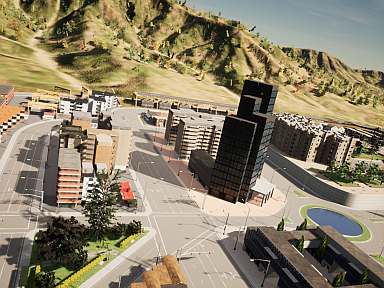
\includegraphics[width=\textwidth]{figures/carla-img-example.png}
        \caption{Example of a generated image}\label{fig:carla-1}
    \end{subfigure}
    \begin{subfigure}{0.45\textwidth}
        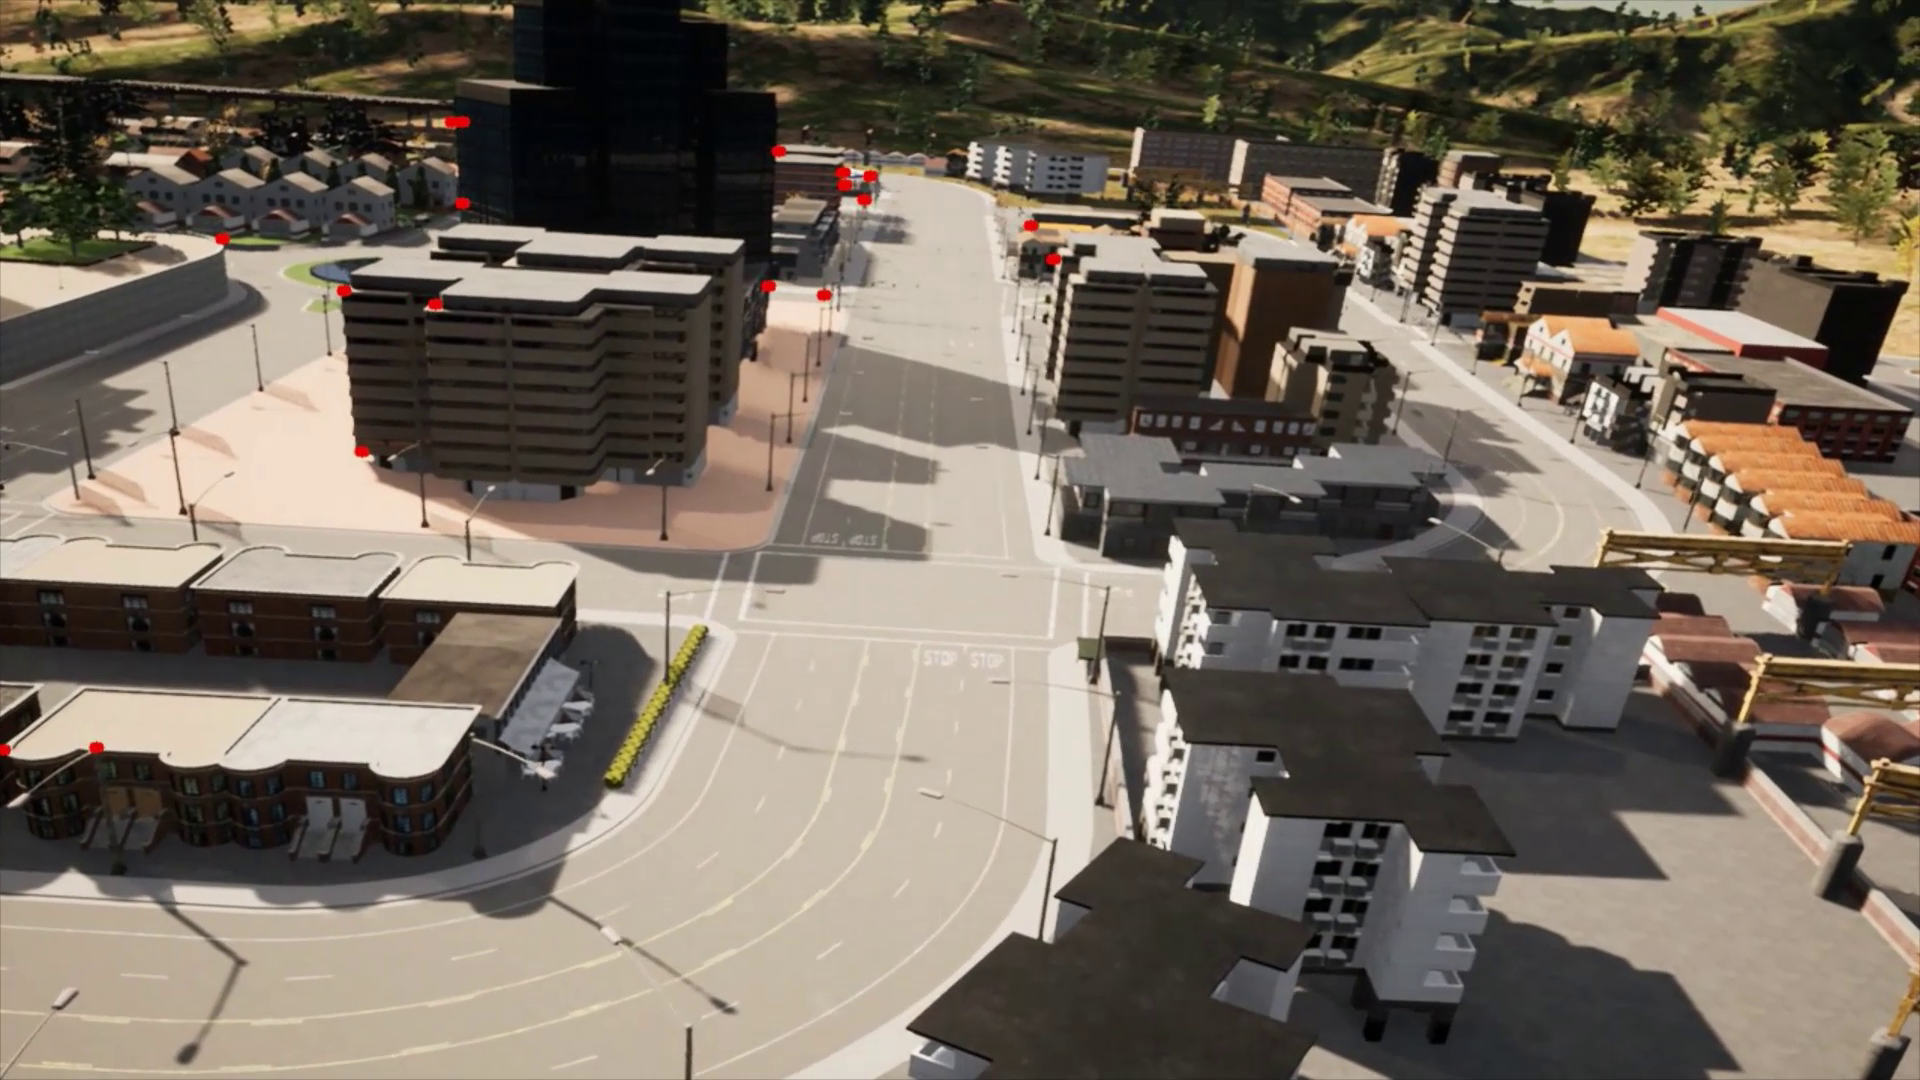
\includegraphics[width=\textwidth]{figures/carla-img-corner.png}
        \caption{Example of the detected corners}\label{fig:carla-2}
    \end{subfigure}
    \caption{Synthetic images}\label{fig:carla}
\end{figure}

In this case, the estimated and the actual 2-D position is shown in Figure~\ref{fig:carla-path} and the accumulated error as a function of the distance travelled in Figure~\ref{fig:carla-error}. I want to highlight that in this case, I only had 10\si{\second} of data to run the simulation.

\begin{figure}[H]
    \centering
    \begin{subfigure}{0.45\textwidth}
        \includesvg[width=0.8\textwidth, inkscapelatex=false]{figures/carla/carla-path}
        \caption{Flight path of CARLA based}\label{fig:carla-path}
    \end{subfigure}
    \begin{subfigure}{0.45\textwidth}
        \includesvg[width=0.8\textwidth, inkscapelatex=false]{figures/carla/carla-path-error}
        \caption{Relative error of CARLA based}\label{fig:carla-error}
    \end{subfigure}
\end{figure}

\begin{figure}[H]
    \centering
    \begin{subfigure}{0.3\textwidth}
        \includesvg[width=\textwidth, inkscapelatex=false]{figures/carla/X-4}
        \caption{CARLA based---X}
    \end{subfigure}
    \hfill
    \begin{subfigure}{0.3\textwidth}
        \includesvg[width=\textwidth, inkscapelatex=false]{figures/carla/Y-4}
        \caption{CARLA based---Y}
    \end{subfigure}
    \hfill
    \begin{subfigure}{0.3\textwidth}
        \includesvg[width=\textwidth, inkscapelatex=false]{figures/carla/Z-4}
        \caption{CARLA based---Z}
    \end{subfigure}
    \caption{CARLA based---position}\label{fig:carla-pos}
\end{figure}

\begin{figure}[H]
    \centering
    \begin{subfigure}{0.3\textwidth}
        \includesvg[width=\textwidth, inkscapelatex=false]{figures/carla/roll-4}
        \caption{CARLA based---roll}
    \end{subfigure}
    \hfill
    \begin{subfigure}{0.3\textwidth}
        \includesvg[width=\textwidth, inkscapelatex=false]{figures/carla/pitch-4}
        \caption{CARLA based---pitch}
    \end{subfigure}
    \hfill
    \begin{subfigure}{0.3\textwidth}
        \includesvg[width=\textwidth, inkscapelatex=false]{figures/carla/yaw-4}
        \caption{CARLA based---yaw}
    \end{subfigure}
    \caption{CARLA based---Euler angles}\label{fig:carla-euler}
\end{figure}

\begin{figure}[H]
    \centering
    \begin{subfigure}{0.3\textwidth}
        \includesvg[width=\textwidth, inkscapelatex=false]{figures/carla/vbx-4}
        \caption{CARLA based---$v_x$}
    \end{subfigure}
    \hfill
    \begin{subfigure}{0.3\textwidth}
        \includesvg[width=\textwidth, inkscapelatex=false]{figures/carla/vby-4}
        \caption{CARLA based---$v_y$}
    \end{subfigure}
    \hfill
    \begin{subfigure}{0.3\textwidth}
        \includesvg[width=\textwidth, inkscapelatex=false]{figures/carla/vbz-4}
        \caption{CARLA based---$v_z$}
    \end{subfigure}
    \caption{CARLA based---velocity}\label{fig:carla-vel}
\end{figure}

\begin{figure}[H]
    \centering
    \begin{subfigure}{0.3\textwidth}
        \includesvg[width=\textwidth, inkscapelatex=false]{figures/carla/abx-4}
        \caption{CARLA based---$a_{b,x}$}
    \end{subfigure}
    \hfill
    \begin{subfigure}{0.3\textwidth}
        \includesvg[width=\textwidth, inkscapelatex=false]{figures/carla/aby-4}
        \caption{CARLA based---$a_{b,y}$}
    \end{subfigure}
    \hfill
    \begin{subfigure}{0.3\textwidth}
        \includesvg[width=\textwidth, inkscapelatex=false]{figures/carla/abz-4}
        \caption{CARLA based---$a_{b,z}$}
    \end{subfigure}
    \caption{CARLA based---acceleration bias}\label{fig:carla-abias}
\end{figure}

\begin{figure}[H]
    \centering
    \begin{subfigure}{0.3\textwidth}
        \includesvg[width=\textwidth, inkscapelatex=false]{figures/carla/wbx-4}
        \caption{CARLA based---$\omega_{b,x}$}
    \end{subfigure}
    \hfill
    \begin{subfigure}{0.3\textwidth}
        \includesvg[width=\textwidth, inkscapelatex=false]{figures/carla/wby-4}
        \caption{CARLA based---$\omega_{b,y}$}
    \end{subfigure}
    \hfill
    \begin{subfigure}{0.3\textwidth}
        \includesvg[width=\textwidth, inkscapelatex=false]{figures/carla/wbz-4}
        \caption{CARLA based---$\omega_{b,z}$}
    \end{subfigure}
    \caption{CARLA based---gyroscope bias}\label{fig:carla-gbias}
\end{figure}

In this case, all of the position and velocity values are degraded significantly through time, but the angles remain close to the true values. It's important to note that this was the first try to use this algorithm with a real image processing algorithm, hence, further developments and improvements are needed to achieve better results. Moreover, the ESKF estimates did not have time to converge, therefore, the results are not as good as in the previous cases. The accumulated 2-D error remains under 6\% of the travelled distance at the end of the simulation.

\subsection{Root mean square error (RMSE)} 

RMSE is a commonly used metric for evaluating the performance of regression models or estimating the quality of predictions. It is a remarkable approach to formalize and numerically express the error between ideal $a$ and observed $\hat{a}$ values. Mathematically, it can be expressed as:
\begin{equation}
    RMSE(a)=\sqrt{\frac{1}{N}\sum_{i=1}^N(\hat{a}-a)^2}
\end{equation}

As a final point of the performance analysis, the RMSE of the ESKF states are presented in Table~\ref{tab:rmse}.

\begin{table}[!ht]
    \centering
    \begin{tabular}{| c | c | c | c | c |}
        \hline
        Variable & Straight\& level & Straight\& descending & Zig-zag\& level & CARLA \\ 
        \hline
        X & 3.19\si{\meter} & 3.01\si{\meter} & 10.76\si{\meter} & 0.61\si{\meter} \\
        Y & 0.14\si{\meter} & 2.71\si{\meter} & 2.97\si{\meter} & 4.01\si{\meter} \\
        Z & 0.35\si{\meter} & 0.34\si{\meter} & 1.77\si{\meter} & 1.1\si{\meter}\\ 
        \hline
        $\phi$ & $20.52^\circ$ & $38.75^\circ$ & $25.39^\circ$ & $26.87^\circ$\\
        $\theta$ & $29.46^\circ$ & $30.56^\circ$ & $31.62^\circ$ & $17.37^\circ$ \\
        $\psi$ & $26.82^\circ$ & $44.94^\circ$ & $36.87^\circ$ & $13.84^\circ$ \\ 
        \hline
        $v_x$ & 0.204\si{\meter}/\si{\s} & 0.202\si{\meter}/\si{\s} & 0.546\si{\meter}/\si{\s} & 0.383\si{\meter}/\si{\s} \\
        $v_y$ & 0.173\si{\meter}/\si{\s} & 0.374\si{\meter}/\si{\s} & 0.269\si{\meter}/\si{\s} & 1.209\si{\meter}/\si{\s} \\
        $v_z$ & 0.315\si{\meter}/\si{\s} & 0.284\si{\meter}/\si{\s} & 0.333\si{\meter}/\si{\s} & 0.118\si{\meter}/\si{\s} \\
        \hline
        $a_{b, x}$ & 0.074\si{\meter}/\si{\s\squared} & 0.085\si{\meter}/\si{\s\squared} & 0.087\si{\meter}/\si{\s\squared} & $\approx$0\si{\meter}/\si{\s\squared} \\
        $a_{b, y}$ & 0.083\si{\meter}/\si{\s\squared} & 0.074\si{\meter}/\si{\s\squared} & 0.077\si{\meter}/\si{\s\squared} & $\approx$0\si{\meter}/\si{\s\squared} \\
        $a_{b, z}$ & 0.006\si{\meter}/\si{\s\squared} & 0.078\si{\meter}/\si{\s\squared} & 0.083\si{\meter}/\si{\s\squared} & $\approx$0\si{\meter}/\si{\s\squared} \\ 
        \hline
        $\omega_{b, x}$ & $0.35^\circ/\si{\s}$ & $0.35^\circ/\si{\s}$ & $0.35^\circ/\si{\s}$ & $\approx 0^\circ/\si{\s}$ \\
        $\omega_{b, y}$ & $0.43^\circ/\si{\s}$ & $0.43^\circ/\si{\s}$ & $0.43^\circ/\si{\s}$ & $\approx 0^\circ/\si{\s}$ \\
        $\omega_{b, z}$ & $0.43^\circ/\si{\s}$ & $0.44^\circ/\si{\s}$ & $0.43^\circ/\si{\s}$ & $\approx 0^\circ/\si{\s}$ \\
        \hline
    \end{tabular}
    \caption{RMSE values}
    \label{tab:rmse}
\end{table}